\section{积分形式}
\label{sec:ivp-integral}

解析解的方法到此为止，绝大多数方程不属于上面这些类型。没有公式时还能怎样谈论解？微分方程约束的是导数，而导数对曲线的小改动极其敏感。把方程两边从起点积分，导数就消失了，得到的新形式更容易分析。

\paragraph{累积变化}
设$\bm{x}$是解。状态在$[t_0,t]$上的变化，是沿途所有瞬时变化率的累积，而瞬时变化率就是方程的右端。于是
\begin{equation}
 \bm{x}(t)=\bm{x}_0+\int_{t_0}^{t}\bm{f}\bigl(s,\bm{x}(s)\bigr)\,\mathrm{d}s.
 \label{eq:ivp-integral}
\end{equation}
这里的积分对向量逐分量进行，$t<t_0$时按有向积分理解。式~\eqref{eq:ivp-integral}称为初值问题的\term{积分形式}（integral form）。

用Logistic方程的解检验这个读法。沿解$x=\mathrm{e}^{s}/(9+\mathrm{e}^{s})$的速度是$x(1-x)=9\mathrm{e}^{s}/(9+\mathrm{e}^{s})^2$，它的原函数是$-9/(9+\mathrm{e}^{s})$，所以从$0$累积到$\ln 9$的面积是
\[
 \int_0^{\ln 9}\frac{9\mathrm{e}^{s}}{(9+\mathrm{e}^{s})^2}\,\mathrm{d}s
 =-\frac{9}{18}+\frac{9}{10}=0.4.
\]
这正好等于$x(\ln 9)-x(0)=0.5-0.1$，如图~\ref{fig:ivp-integral-area}(a)(b)所示。

\begin{BookInlineFigure}
 \centering
 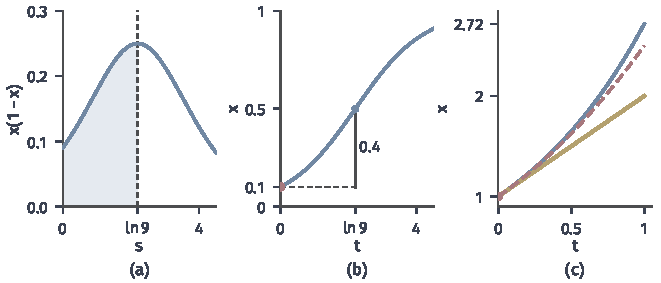
\includegraphics[width=112mm]{figures/06-differential-equations/01-ordinary-differential-equations/matplotlib/ivp-integral-area/figure.pdf}
 \caption{积分形式的读法。(a)沿Logistic解的速度曲线$x(1-x)$，浅蓝区是从$0$到$\ln 9$的累积，面积为$0.4$。(b)解曲线在同一段上的增量恰为$0.4$。(c)方程$\dot{x}=x$，$x(0)=1$：黄线是试探曲线$1+t$，红色虚线是把它代入式~\eqref{eq:ivp-integral}右端得到的$1+t+t^2/2$，蓝线是真解$\mathrm{e}^{t}$，只有真解代入后不变。}
 \label{fig:ivp-integral-area}
\end{BookInlineFigure}

\paragraph{两种形式等价}
微分形式要求曲线可微，积分形式只要求右端能积分。连续右端下，两者描述同样的曲线。

\begin{theorem}[微分形式与积分形式的等价性]
 \label{thm:ivp-integral-equivalence}
 设$\bm{f}$在$T\times\bm{D}$上连续，$I\subseteq T$是包含$t_0$的区间，$\bm{x}:I\to\bm{D}$连续。则$\bm{x}$是初值问题~\eqref{eq:ivp-ivp}在$I$上的经典解，当且仅当$\bm{x}$在$I$上处处满足积分方程~\eqref{eq:ivp-integral}。
\end{theorem}

\begin{proof}
 设$\bm{x}$是经典解。由第~\ref{sec:ivp-verification}节的说明，$\dot{\bm{x}}(s)=\bm{f}(s,\bm{x}(s))$连续。对每个分量用微积分基本定理，
 \[
 \bm{x}(t)-\bm{x}(t_0)=\int_{t_0}^{t}\dot{\bm{x}}(s)\,\mathrm{d}s
 =\int_{t_0}^{t}\bm{f}\bigl(s,\bm{x}(s)\bigr)\,\mathrm{d}s,
 \]
 再代入$\bm{x}(t_0)=\bm{x}_0$，就得到式~\eqref{eq:ivp-integral}。

 反过来，设连续曲线$\bm{x}$满足式~\eqref{eq:ivp-integral}。$\bm{f}$连续、$\bm{x}$连续，所以被积函数$s\mapsto\bm{f}(s,\bm{x}(s))$连续。由微积分基本定理的另一方向，式~\eqref{eq:ivp-integral}右端关于$t$连续可微，导数等于$\bm{f}(t,\bm{x}(t))$，这就是微分方程。令$t=t_0$，积分为零，得到初值。
\end{proof}

定理用到的是连续函数的微积分基本定理，可参考\BookChapterRef{chap:univariate-integration}{卷一第7章“一元函数的积分”}。证明里连续性出现了两次：$\bm{f}$连续让被积函数连续，从而让变上限积分可导。若$\bm{f}$在时间上有跳变，这一步就会失败，下一节处理这种情形。

\paragraph{积分形式保留了初值}
微分方程$\dot{\bm{x}}=\bm{f}(t,\bm{x})$本身不知道从哪里出发，初值要另外写。积分方程把初值写在了式子里：$\bm{x}_0$就是右端的第一项，令$t=t_0$立刻读出。例如在$\dot{x}=\cos t$中，$\sin t$和$\sin t+5$是同一个微分方程的两条解，而积分方程$x(t)=x_0+\int_0^t\cos s\,\mathrm{d}s$对给定的$x_0$只有一条解。

\paragraph{解是自洽的曲线}
式~\eqref{eq:ivp-integral}还有一个结构上的特点：未知曲线同时出现在两边。曲线决定沿途的速度，速度累积后必须重新给出同一条曲线。若把右端看作把一条曲线变成另一条曲线的映射，解就是这个映射的不动点。

拿方程$\dot{x}=x$，$x(0)=1$来试。积分方程是$x(t)=1+\int_0^t x(s)\,\mathrm{d}s$。把试探曲线$x(t)=1+t$代入右端，得到
\[
 1+\int_0^t(1+s)\,\mathrm{d}s=1+t+\frac{t^2}{2},
\]
与试探曲线不同，所以$1+t$不是解。把$\mathrm{e}^{t}$代入，右端是$1+(\mathrm{e}^{t}-1)=\mathrm{e}^{t}$，映射后不变。图~\ref{fig:ivp-integral-area}(c)比较了这三条曲线。解的存在性和唯一性由第~\ref{chap:ode-existence-continuation}章从这个不动点结构出发证明，那里的Picard迭代正是反复做这种代入。

\paragraph{积分比导数温和}
积分形式好用的另一个原因，是积分对小扰动不敏感，而导数恰好相反。取
\[
 \delta(t)=\varepsilon\sin\frac{t}{\varepsilon^2},
\]
$\varepsilon$很小时，这是一个幅度为$\varepsilon$的高频抖动。它的导数和变上限积分分别是
\[
 \dot{\delta}(t)=\frac{1}{\varepsilon}\cos\frac{t}{\varepsilon^2},\qquad
 \int_0^t\delta(s)\,\mathrm{d}s=\varepsilon^3\Bigl(1-\cos\frac{t}{\varepsilon^2}\Bigr).
\]
曲线本身的差距是$\varepsilon$，导数的差距却有$1/\varepsilon$，积分的差距只有$2\varepsilon^3$。图~\ref{fig:ivp-integral-smoothing}取$\varepsilon=0.2$，三个幅度是$0.2$、$5$和$0.016$。

\begin{BookInlineFigure}
 \centering
 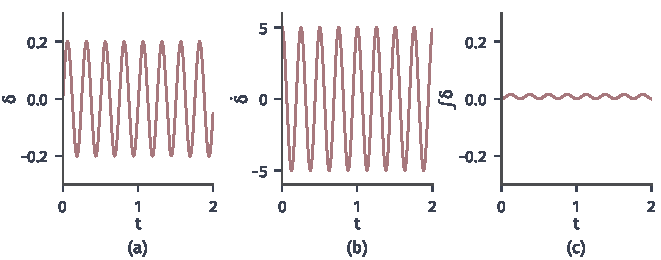
\includegraphics[width=112mm]{figures/06-differential-equations/01-ordinary-differential-equations/matplotlib/ivp-integral-smoothing/figure.pdf}
 \caption{高频小扰动$\delta(t)=\varepsilon\sin(t/\varepsilon^2)$，$\varepsilon=0.2$。(a)扰动本身，幅度$0.2$。(b)导数，幅度$5$。(c)变上限积分，幅度不超过$2\varepsilon^3=0.016$，(a)和(c)使用相同的纵轴。}
 \label{fig:ivp-integral-smoothing}
\end{BookInlineFigure}

这个对比说明了两种形式的不同用处。两条曲线接近时，它们的导数可能相差很大，所以在微分形式中无法比较；积分形式中，两边都只涉及曲线本身的值。设$\bm{x}$、$\tilde{\bm{x}}$分别是初值$\bm{x}_0$、$\tilde{\bm{x}}_0$对应的解，相减得到
\begin{equation}
 \bm{x}(t)-\tilde{\bm{x}}(t)=\bm{x}_0-\tilde{\bm{x}}_0+\int_{t_0}^{t}\bigl[\bm{f}(s,\bm{x}(s))-\bm{f}(s,\tilde{\bm{x}}(s))\bigr]\,\mathrm{d}s,
 \label{eq:ivp-integral-difference}
\end{equation}
差值完全由差值控制，不出现导数。第~\ref{chap:ode-sensitivity}章从这个等式出发估计数据误差的影响。

\paragraph{解的光滑性}
积分形式也回答了解有多光滑。若$\bm{f}$连续，由定理~\ref{thm:ivp-integral-equivalence}，$\bm{x}$连续可微。若$\bm{f}$进一步是$k$次连续可微的，可以一阶一阶往上推。假设已知$\bm{x}$是$j$次连续可微的，$j\leq k$，则复合函数$s\mapsto\bm{f}(s,\bm{x}(s))$也是$j$次连续可微的，而$\bm{x}$是它的变上限积分加常数，所以$\bm{x}$是$j+1$次连续可微的。从$j=1$推到$j=k$，得到$\bm{x}$是$k+1$次连续可微的：解总比右端多一阶光滑。Logistic方程的右端是多项式，所以解是无穷次可微的。

下表归纳两种形式的不同之处。
\begin{BookInlineTable}
 \centering
 \caption{微分形式与积分形式}
 \label{tab:ivp-two-forms}
 \begin{tabular}{lll}
 \toprule
 比较项 & 微分形式 & 积分形式 \\
 \midrule
 对曲线的要求 & 可微 & 被积函数可积 \\
 初值 & 另外给出 & 写在式子里 \\
 对小扰动 & 导数可以很大 & 积分很小 \\
 适合做什么 & 代入检验 & 证明与误差估计 \\
 \bottomrule
 \end{tabular}
\end{BookInlineTable}
